\documentclass{beamer}
%~ \documentclass[hyperref={pdfpagelabels=false}]{beamer}

\usepackage[ngerman,english]{babel}
\usepackage[utf8]{inputenc}
\usepackage{lmodern}
\usepackage{beamerthemeshadow}

%\usepackage{la}
\usepackage[T1]{fontenc}

\definecolor{mygreen}{rgb}{0,0.5,0}
\usecolortheme[named=mygreen]{structure}

\usepackage{listings}
\lstdefinestyle{sharpc}{language=[Sharp]C, frame=lr, rulecolor=\color{blue!80!black}}

\title{A Unified Framework for Digital Image Processing in Computer Vision and Remote Sensing}
\author{
Carsten Brandt,
Ludmilla Brandt,
Akarsh Seggemu,\\
Onur Ünal,
Marcus Zepp
}
\date{\today}

\newcommand{\beginbackup}{
   \newcounter{framenumbervorappendix}
   \setcounter{framenumbervorappendix}{\value{framenumber}}
}
\newcommand{\backupend}{
   \addtocounter{framenumbervorappendix}{-\value{framenumber}}
   \addtocounter{framenumber}{\value{framenumbervorappendix}}
}

% table of contents should not show subsections
\setcounter{tocdepth}{1}

% allow using color
\usepackage{color}
\usepackage{xcolor}

% the lstlistings package
\usepackage{listings}
% highlighting lines in listings
\usepackage{linehighlight}

% set colors for code background and highlighting
\definecolor{codehighlight}{rgb}{0.95,0.8,0.8}
\definecolor{codebackground}{rgb}{0.95,0.95,0.95}

%~ % Dadurch wird verhindert, dass die Navigationsleiste angezeigt wird.
%~ \setbeamertemplate{navigation symbols}{}
\setbeamertemplate{footline}{
  \leavevmode%
  \hbox{%
	  \begin{beamercolorbox}[wd=.75\paperwidth,ht=2.25ex,dp=1ex,center]{author in head/foot}%
			\usebeamerfont{author in head/foot}\insertshortauthor%~~(\insertshortinstitute)
	  \end{beamercolorbox}%
%	  \begin{beamercolorbox}[wd=.5\paperwidth,ht=2.25ex,dp=1ex,center]{title in head/foot}%
%			\usebeamerfont{title in head/foot}\insertshorttitle
%	  \end{beamercolorbox}%
	  \begin{beamercolorbox}[wd=.25\paperwidth,ht=2.25ex,dp=1ex,right]{date in head/foot}%
			\usebeamerfont{date in head/foot}\insertshortdate{}\hspace*{2em}
			\insertframenumber{} / \inserttotalframenumber % hier hat's sich geändert
	  \end{beamercolorbox}
	  }%
  \vskip0pt%
}

% http://tex.stackexchange.com/questions/16357/how-can-i-position-an-image-in-an-arbitrary-position-in-beamer
\usepackage{tikz}
%\usetikzlibrary{calc, trees, positioning, arrows, shapes, shapes.multipart, shadows, matrix, decorations.pathreplacing, decorations.pathmorphing}
\usetikzlibrary{arrows}%, shapes, shapes.multipart}

% creating histograms
% http://tex.stackexchange.com/questions/130531/automatic-binning-of-histogram-using-raw-gnuplot-in-pgfplot
% \usepackage{pgfplots}
% \usepackage{pgfplotstable}
% \usetikzlibrary{external}
% \tikzexternalize
% \tikzset{external/force remake}
% %\pgfplotsset{compat=1.8}


\tikzset{
  every boverlay node/.style={
    draw=black,fill=white,rounded corners,anchor=north west,
  },
}
\tikzset{
  every overlay node/.style={
    %draw=white,fill=white,rounded corners,anchor=north west,
    anchor=north west
  },
}
% Usage:
% \tikzoverlay at (-1cm,-5cm) {content};
% or
% \tikzoverlay[text width=5cm] at (-1cm,-5cm) {content};
\def\tikzboverlay{%
   \tikz[baseline,overlay]\node[every boverlay node]
}%
\def\tikzoverlay{%
   \tikz[baseline,overlay]\node[every overlay node]
}%

\usetheme{default}
% default, bars, boxes, classic, lined, plain, shadow, sidebar, split, tree
% Berlin, Darmstadt, Dresden, Frankfurt, Goettingen, Hannover, Ilmenau, Luebeck, . . . , Warsaw

\usepackage{pdfpcnotes}

% Notizen zu jeder Folie auf zweitem Bildschirm anzeigen
%~ \setbeameroption{show notes on second screen = right}
% Notizen beliebig innerhalb des Frames setzen:
% 1 (...)
% 2 \note{Hier eine Notiz}
% 3 (...)
% 4 \note[item]{und noch eine Notiz , diesmal geordnet}
% 5 (...)



\definecolor{codehighlight}{rgb}{0.95,0.8,0.8}
\definecolor{codebackground}{rgb}{0.95,0.95,0.95}

\definecolor{exercisecolor}{rgb}{0.63, 0.90, 1.00}

\definecolor{lightgrey}{rgb}{0.9,0.9,0.9}
\definecolor{mygreen}{rgb}{0,0.6,0}
\definecolor{mygray}{rgb}{0.5,0.5,0.5}
\definecolor{mymauve}{rgb}{0.58,0,0.82}

\lstset{ %
%	backgroundcolor=\color{lightgrey},   % choose the background color; you must add \usepackage{color} or \usepackage{xcolor}
	breakatwhitespace=true,          % sets if automatic breaks should only happen at whitespace
	breaklines=true,                 % sets automatic line breaking
	captionpos=b,                    % sets the caption-position to bottom
%	deletekeywords={...},            % if you want to delete keywords from the given language
%	escapeinside={\%*}{*)},          % if you want to add LaTeX within your code
%	extendedchars=true,              % lets you use non-ASCII characters; for 8-bits encodings only, does not work with UTF-8
	frame=single,                    % adds a frame around the code
	keepspaces=true,                 % keeps spaces in text, useful for keeping indentation of code (possibly needs columns=flexible)
	language=C++,                    % the language of the code
	morekeywords={*,php,class,extends,public,protected,private,foreach,if,else,elseif,%
		function,return,new,echo,endforeach,vector,Context
	},            % if you want to add more keywords to the set
	numbers=left,                    % where to put the line-numbers; possible values are (none, left, right)
	numbersep=10pt,                   % how far the line-numbers are from the code
%	rulecolor=\color{black},         % if not set, the frame-color may be changed on line-breaks within not-black text (e.g. comments (green here))
	showspaces=false,                % show spaces everywhere adding particular underscores; it overrides 'showstringspaces'
	showstringspaces=false,          % underline spaces within strings only
	showtabs=false,                  % show tabs within strings adding particular underscores
	stepnumber=1,                    % the step between two line-numbers. If it's 1, each line will be numbered
	tabsize=4,                       % sets default tabsize to 2 spaces
%	title=\lstname                   % show the filename of files included with \lstinputlisting; also try caption instead of title
	basicstyle=\footnotesize\ttfamily,
	keywordstyle=\bfseries\color{green!40!black},
	commentstyle=\color{purple!40!black},
	identifierstyle=\color{black},
	stringstyle=\color{orange},
	numberstyle=\tiny\color{mygray}, % the style that is used for the line-numbers
}

%  \beamersetuncovermixins{\opaqueness<1>{25}}{\opaqueness<2->{15}}
%  sorgt dafuer das die Elemente die erst noch (zukuenftig) kommen
%  nur schwach angedeutet erscheinen
\beamersetuncovermixins{\opaqueness<1>{25}}{\opaqueness<2->{15}}
% klappt auch bei Tabellen, wenn teTeX verwendet wird\ldots

\begin{document}


\begin{frame}
	\titlepage
\end{frame}

\begin{frame}
	\tableofcontents  \pnote{}
\end{frame}

% Vor jedem Abschnitt automatisch Inhaltsverzeichnis anzeigen:
\AtBeginSection []{
\begin{frame}
	\tableofcontents [currentsection]

	\pnote{
		notes go here...
	}
\end{frame}
}

%---------------------------------------------------------------------------------------------------------------------------------------------
\section{Organisation}
\subsection{Gitlab}
\begin{frame}{Gitlab}

	\Large
	\begin{itemize}
		\item A private and free Github \pause
		\item Share and version code \pause
		\item Issue/Task tracking + Milestones \pause
		\item Merge Requests/Pull Requests
	\end{itemize}

	\pnote{
		- private, free github clone \\
		- versioning is essential in software projects \\
		- it also provides issues and milestones \\
		- Programming workflow with pull requests is common in open source \\
		- git because we want to transfer to github later

	}

\end{frame}

\subsection{Gitlab Issues}
\begin{frame}{Gitlab Issues}
	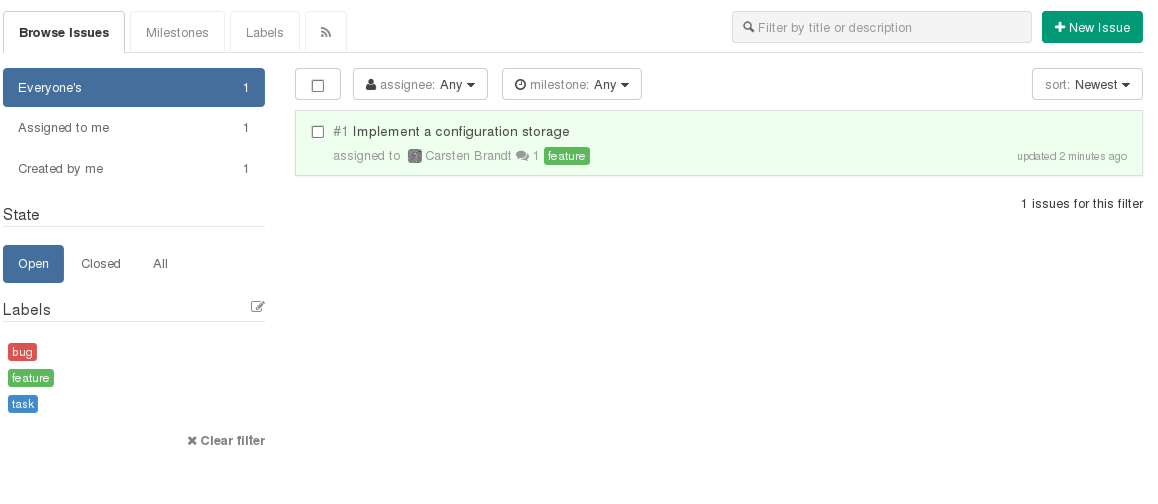
\includegraphics[width=\textwidth]{images/gitlab_issues}

	\pnote{
		- planning by creating issues, assign to milestone \\
		- discussion per ticket/topic, all in one place \\
		- tags/labels  bug, feature, task, urgent, etc... \\
	}
\end{frame}
\begin{frame}{Gitlab Issues}
	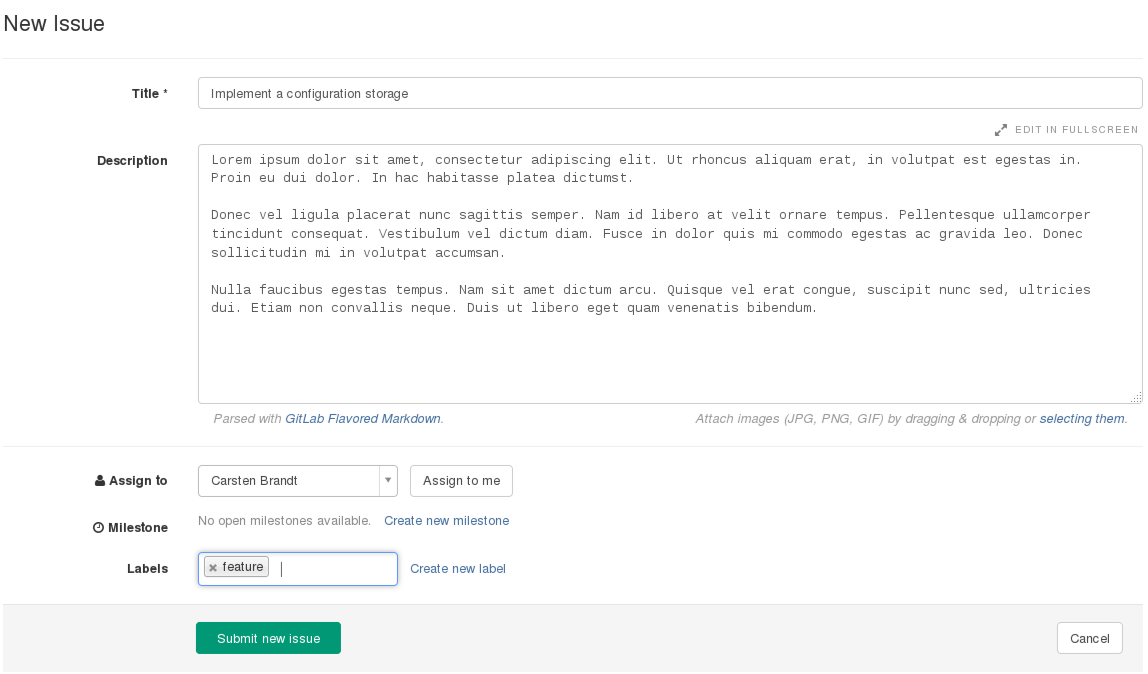
\includegraphics[width=\textwidth]{images/gitlab_new_issue}

	\pnote{
		- short title, issues should be small \\
		- assignees \\
		- due for a milestone \\
		- tagged with labels
	}
\end{frame}

\subsection{Gitlab Merge Requests}
\begin{frame}{Gitlab Merge Requests}

	\begin{itemize}
		\item Work on branches \pause
		\item never push to master directly \pause
		\item code review \pause
		\item better quality \pause
		\item people know about changes
	\end{itemize}

	\pnote{
		- work on branches, master always stable \\
		- never push to master \\
		- code review helps writing cleaner code and spot problems\\
		- more eyes see more \\
		- => better quality \\
		- better team integration, ppl aware of changes \\
	}

\end{frame}
\begin{frame}{Gitlab Merge Requests}
	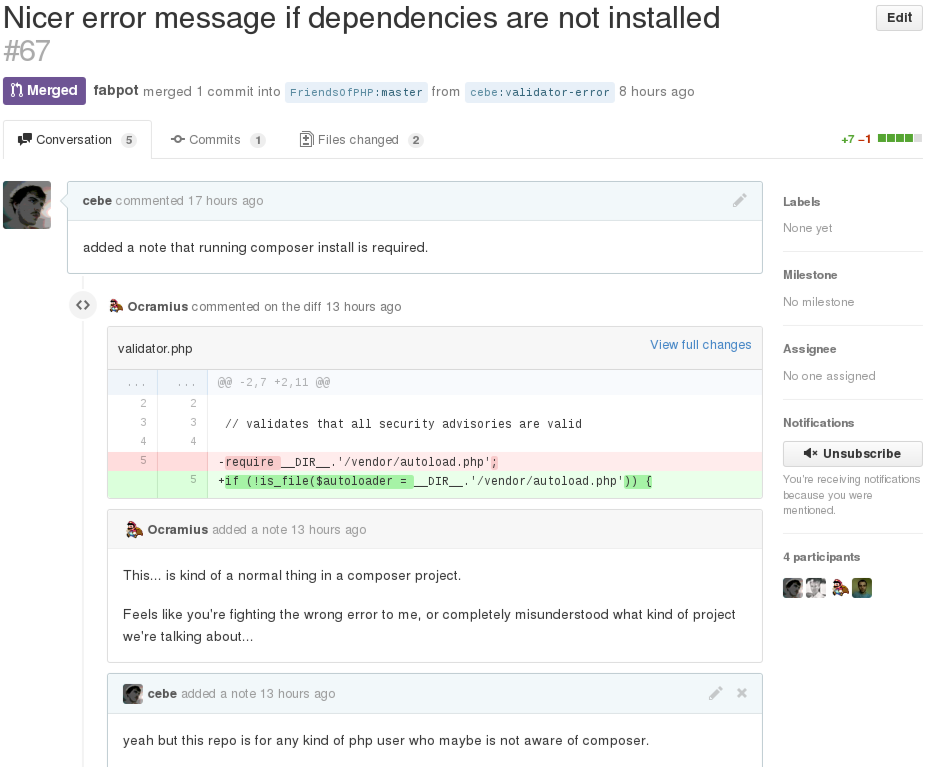
\includegraphics[width=\textwidth]{images/gitlab_pr}

	\pnote{
		- example from github \\
		- send PR, discuss it
	}
\end{frame}

\begin{frame}{Gitlab Merge Requests}
	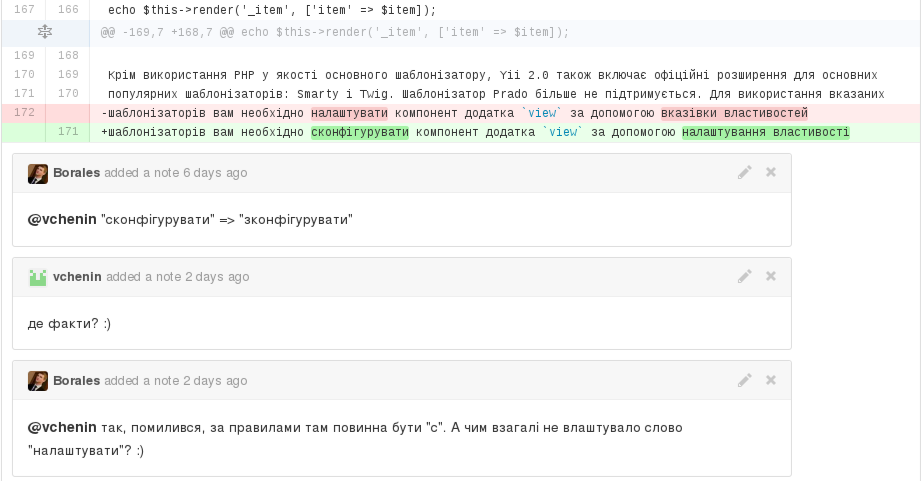
\includegraphics[width=\textwidth]{images/gitlab_pr_comment}

	\pnote{
		- discussion\\
	}
\end{frame}

\begin{frame}{Gitlab Merge Requests}
	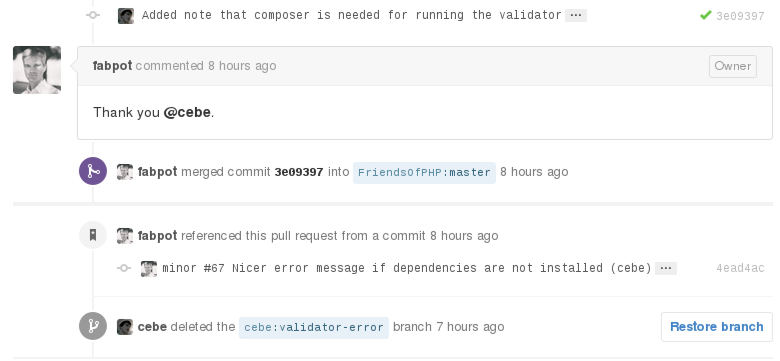
\includegraphics[width=\textwidth]{images/gitlab_pr_merge}

	\pnote{
		- merged if all fine\\
	}
\end{frame}


\section{System Overview}

\begin{frame}{Requirements}

	\begin{itemize}
		\item Plattform independent with linux as primary target \pause
		\item GUI and Command-line mode \pause
		\item Graph based workflow design \pause
		\item No realtime needed \pause
		\item Module/Plugin model \pause
		\item Logging \pause
		\item Arbitrary data sources and sinks
	\end{itemize}

\end{frame}

\begin{frame}{System Overview}

	\begin{tikzpicture}
		\tikzstyle{mybox}=[draw,minimum width=2cm,minimum height=1cm,rounded corners]
		\node[mybox] (gui)  at (-2.5,0) {GUI Interface};
		\node[mybox] (console) at (2.5,0) {Console Interface};
		\node[mybox,minimum width=10cm] (framework) at (0,-2) {Processing Framework};

		\node[mybox] (config) at (-3,-4) {Configuration Storage};
		\node[mybox] (module1) at (1,-4) {Module $1$};
		\node at (2.5,-4) {\dots};
		\node[mybox] (modulen) at (4,-4) {Module $n$};

		\draw[->] (gui) -- (framework.north);
		\draw[->] (console) -- (framework);
		\draw (framework) -- (module1);
		\draw (framework) -- (modulen);
		\draw (framework) -- (config);

	\end{tikzpicture}

\end{frame}

\subsection{Framework}
\begin{frame}{Framework}

	Functionality:
	\begin{itemize}
		\item load/save chain config
		\item run chain
		\item sanity check of chain before run
	\end{itemize}

\end{frame}

\subsection{GUI}
\begin{frame}{GUI}

	GUI Elements
	Functionality:
	\begin{itemize}
		\item load/save chain config
		\item add/rm modules
 		\item link/unlink modules
  		\item run chain
	 	\item sanity check of chain before run
	 	\item display logging information
	\end{itemize}

\end{frame}

\subsection{Configuration Storage}
\begin{frame}{Configuration Storage}

	\Large
	Requirements:

	\vspace{1cm}
	\begin{itemize}
		\item read and writeable by human and machine
		\item ideally simpler than XML
	\end{itemize}

	\pnote{
	- store chain of the modules \\
	- execute in which order and which parameters\\

	- chain can be created by GUI \\
	- but console we must create the file by hand\\

	- XML has too much overhead to write it\\
	}

\end{frame}

\subsection{Modules}
\begin{frame}{Modules}

	Modules provide the processing functionality of the framework.

\pause
	\vspace{1cm}
	\Large
	Consists of
	\begin{itemize}
		\item a meta information file
		\item a library file
	\end{itemize}

\end{frame}

\begin{frame}[fragile,t]{Interface}

	Basic interface:
	\begin{lstlisting}
		void run(vector input, vector output, Context context)
	\end{lstlisting}

	\only<1-3>{
	  \begin{itemize}
		\item<2-> \lstinline|input| and \lstinline|output| are \lstinline|std::vector| of resources described in module meta description
			\pause
		\item<3> \lstinline|context| implements a defined interface to the execution context
			\begin{itemize}
				\item write to logger
				\item open windows
				\item \dots
			\end{itemize}
	  \end{itemize}
	}
	\only<4->{
	  \begin{itemize}
		\item<5-> Image with arbitrary number of channels
			\begin{itemize}
				\item Grayscale, RGB, CMYK, \dots
				\item PolSAR
				\item OpenCV Mat
			\end{itemize}\pause
		\item<6-> integer \pause
		\item<7-> float \pause
		\item<8-> string \pause
		\item<9-> a list of the above \pause
		\item<10-> a map: string $\rightarrow$ one of the above
	  \end{itemize}
	}

\end{frame}



\section{Implementation}
\begin{frame}{Implementation}

	\Large
	\begin{itemize}
		\item Language: C++11
		\item Build Tool: CMake
		\item Libraries: OpenCV, Qt
	\end{itemize}

\end{frame}

\section{Time Schedule}
\begin{frame}{Time Schedule}

	{\Huge Milestones}
	\vspace{1cm}


	\Large
	\begin{tabular}{|c|c|p{5cm}|}
		\hline
		1st	&	26.05.2015	&	Core Framework Basics and Configuration \\ \hline
		2nd	&	09.06.2015	&	Basic Modules \\ \hline
		3rd	&	23.06.2015	&	GUI \\ \hline
		4th	&	07.07.2015	&	Working framework 1.0 \\ \hline
			&	14.07.2015	&	Final Presentation	\\ \hline
	\end{tabular}

\end{frame}





%\beginbackup
%\section{Appendix}

%\begin{frame}
%	\frametitle{Pack-Man}
%...
%\end{frame}

%\backupend

\end{document}
